\documentclass[11pt]{article}
% ---------------------------------------------------------------------------
%  ccint project wrap-up — preamble
%  Compiles with pdfLaTeX (Overleaf default; no configuration needed).
% ---------------------------------------------------------------------------
\usepackage[T1]{fontenc}
\usepackage[utf8]{inputenc}
\usepackage{lmodern}
\usepackage[letterpaper,margin=1in,headheight=14pt]{geometry}
\usepackage{microtype}
\setlength{\emergencystretch}{3em}   % 允许必要时额外伸缩，消除长代码标识符造成的溢出

\usepackage{booktabs}
\usepackage{tabularx}
\usepackage{longtable}
\usepackage{array}
\usepackage{multirow}
\usepackage{amssymb}
\usepackage{amsmath}
\usepackage{enumitem}
\usepackage{fancyhdr}
\usepackage{titlesec}
\usepackage{graphicx}
\graphicspath{{figures/}}
\usepackage{tikz}
\usetikzlibrary{arrows.meta,positioning,calc,fit,backgrounds}
\usepackage[skins,breakable]{tcolorbox}

\usepackage[dvipsnames]{xcolor}
\definecolor{ink}{HTML}{1A1A1A}
\definecolor{accent}{HTML}{1F4E79}
\definecolor{warn}{HTML}{9C4221}
\definecolor{good}{HTML}{22543D}
\definecolor{rule}{HTML}{C8CDD4}
\definecolor{softbg}{HTML}{F4F6F8}
\definecolor{accentbg}{HTML}{EAF0F6}

\usepackage[font=small,labelfont={bf,color=accent},skip=8pt]{caption}

\usepackage[colorlinks=true,linkcolor=accent,urlcolor=accent,citecolor=accent]{hyperref}

% --- headers ---------------------------------------------------------------
\pagestyle{fancy}
\fancyhf{}
\renewcommand{\headrulewidth}{0.4pt}
\fancyhead[L]{\footnotesize\textcolor{accent}{ccint — Canada Cyber Social Intelligence}}
\fancyhead[R]{\footnotesize\thepage}

% --- section styling -------------------------------------------------------
\titleformat{\section}{\Large\bfseries\color{accent}}{\thesection}{0.7em}{}
\titleformat{\subsection}{\large\bfseries\color{ink}}{\thesubsection}{0.6em}{}
\titleformat{\subsubsection}{\normalsize\bfseries\itshape\color{ink}}{}{0em}{}
\titlespacing*{\section}{0pt}{2.2ex plus 1ex minus .2ex}{1.2ex plus .2ex}

% --- table helpers ---------------------------------------------------------
\renewcommand{\arraystretch}{1.18}
\newcolumntype{R}{>{\raggedleft\arraybackslash}X}
\newcolumntype{L}{>{\raggedright\arraybackslash}X}
\newcommand{\hd}[1]{\textbf{#1}}

% --- callout boxes ---------------------------------------------------------
\newtcolorbox{keybox}[1][]{
  enhanced, breakable, colback=accentbg, colframe=accent,
  boxrule=0pt, leftrule=3pt, arc=1pt, left=8pt, right=8pt, top=6pt, bottom=6pt,
  #1}
\newtcolorbox{warnbox}[1][]{
  enhanced, breakable, colback=softbg, colframe=warn,
  boxrule=0pt, leftrule=3pt, arc=1pt, left=8pt, right=8pt, top=6pt, bottom=6pt,
  #1}
\newtcolorbox{plainbox}[1][]{
  enhanced, breakable, colback=softbg, colframe=rule,
  boxrule=0.4pt, arc=1pt, left=8pt, right=8pt, top=6pt, bottom=6pt,
  #1}

% --- inline semantics ------------------------------------------------------
\newcommand{\code}[1]{\texttt{\small #1}}
\newcommand{\yes}{\textcolor{good}{\checkmark}}
\newcommand{\no}{\textcolor{warn}{$\times$}}
\newcommand{\noise}{\textcolor{warn}{noise}}

% --- verbatim-ish code block ----------------------------------------------
\usepackage{fancyvrb}
\DefineVerbatimEnvironment{shell}{Verbatim}
  {fontsize=\small,frame=single,rulecolor=\color{rule},framesep=6pt,
   formatcom=\color{ink}}

\geometry{margin=0.85in,bottom=0.78in}
\setlist{topsep=3pt,itemsep=2pt,parsep=0pt}
\renewcommand{\arraystretch}{1.02}
\linespread{0.96}\selectfont
\renewcommand{\topfraction}{0.92}
\renewcommand{\bottomfraction}{0.75}
\renewcommand{\textfraction}{0.06}
\renewcommand{\floatpagefraction}{0.88}

\begin{document}
\thispagestyle{fancy}
\begin{center}
  \vspace{-0.9cm}
  {\LARGE\bfseries\color{accent}ccint --- Progress Brief}\\[4pt]
  {\large\color{ink} Canada Cyber Social Intelligence: why it is built this
   way, what was built, and where it stands}\\[6pt]
  {\normalsize\color{ink!70} 23 September 2026}
\end{center}
\vspace{0.2cm}

\section*{\color{accent}The question, and what changed about it}

The project began as a longitudinal study: \emph{how does Canada-related
cybersecurity discussion change over time on social media?} A collector runs
continuously, posts are labelled under versioned schemes, and change is tested
statistically.

The first full analysis returned a negative result, and returned it with enough
rigour to be worth something. The largest topic movement in the 30-day window,
\code{data\_breach} at $+22\%$, has $p_{\mathrm{FWER}} = 0.734$ under an
author-level circular-shift null that preserves each author's volume, topic mix
and burstiness while destroying calendar alignment. Empirical power analysis
--- measured by author-pool replication rather than assumed --- puts the
requirement at roughly $8\times$ the current volume.

That result is only interesting if one knows what produced it. Three
explanations were open --- the world, the relevance gate, or the collection
boundary --- and nothing in the system could separate them, because every
figure it produced came from labels it had produced itself. Most of the work
since has been building measurements that can, and the answer was not the
expected one: \textbf{the shortfall is not in the statistics and not mainly in
the labelling --- the platform carries almost no human discussion of these
events at all.}

\section*{\color{accent}Why the system is built this way}

Four commitments shaped every design decision. Each exists to prevent a
specific failure that would be invisible after the fact.

\paragraph{One platform first, and say so.}
An open, documented API with usable historical search and terms permitting
research collection; other platforms were excluded on access grounds rather
than merit. This is a convenience sample, stated rather than hidden, and
measuring what such a sample can show became part of the job.

\paragraph{Labels are versioned and never overwritten.}
Annotation rows are keyed by (post, annotator version) and only ever inserted;
eight annotator versions now coexist over the same corpus and diff row by row.
Otherwise every improvement to the annotator silently rewrites history, and a
shift in topic distribution can never be attributed to the world rather than to
the method.

\paragraph{Raw data is kept verbatim; every number carries provenance.}
Payloads are stored unmodified, and every run and model label records what
produced it, including the SHA-256 of the prompt text. That last part was added
after noticing that a model annotator's output is entirely determined by its
prompt: ``labels are never overwritten'' had preserved the labels while losing
the conditions that made them.

\paragraph{System failure must be distinguishable from social change.}
Every collection path records mode, status, window and counts. The principle
held under test: a token outage appears as 43 \code{partial} runs, not as a
drop in Canadian cyber discussion.

\begin{keybox}
Underlying all four: \textbf{measure before improving.} Repeatedly the
intuitive next step was aimed at the wrong quantity --- tuning the trend score
would have been wasted, relaxing the relevance rules helps but not for the
population that seemed to need it, and the largest prompt improvement in the
project introduced a regression the evaluation set certified as correct.
\end{keybox}

\begin{figure}[htbp]\centering
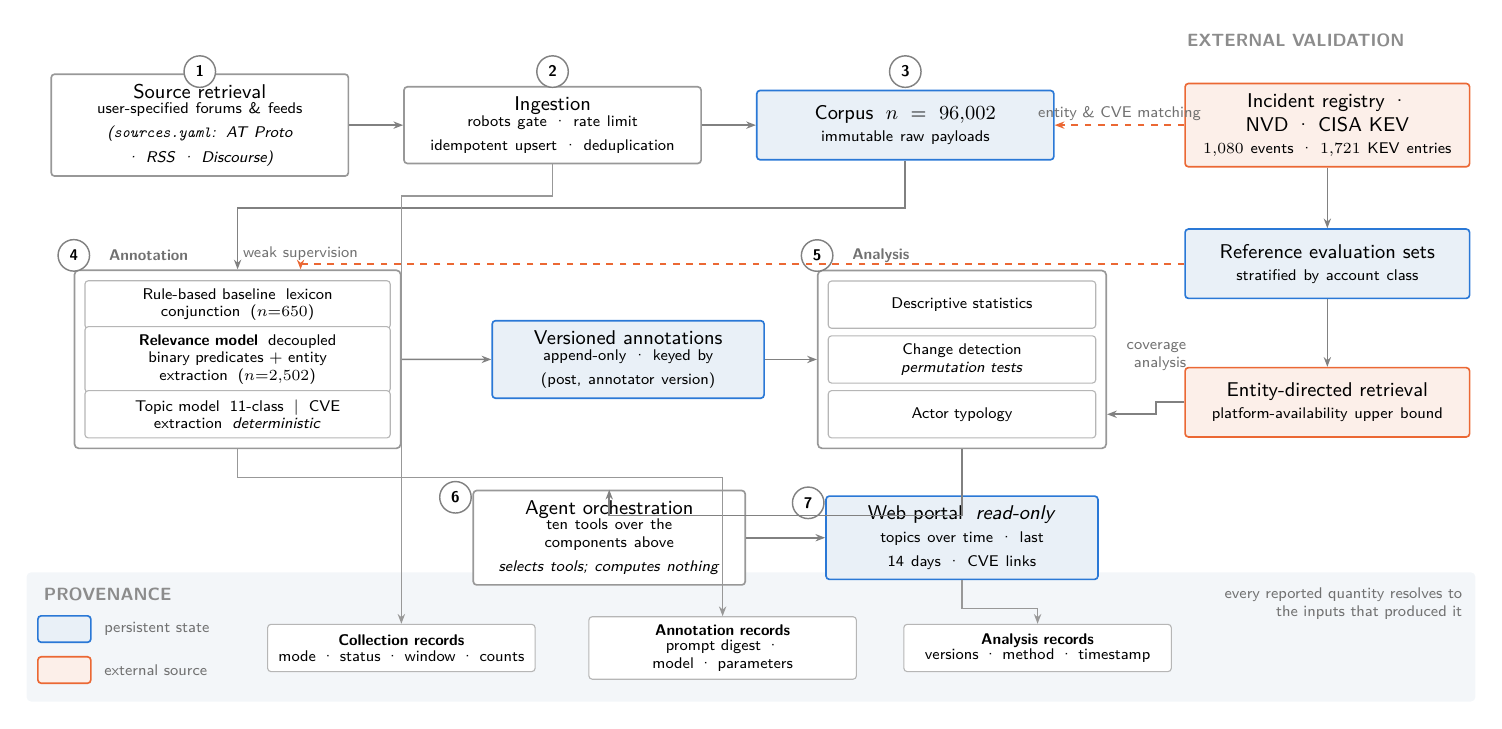
\includegraphics[width=0.70\linewidth]{Architecture.png}
\caption{Processing pipeline. Stages 1--3 acquire and store the corpus, 4
annotates it under coexisting versioned schemes, 5 analyses it, and 6--7 expose
it through a tool-calling agent and a read-only portal. The external-validation
column supplies labels no component of the pipeline produced.}
\label{fig:arch}
\end{figure}

\section*{\color{accent}What was built}

Collection runs in two modes --- a day-by-day backfill and an hourly
incremental --- with idempotent ingestion, stale-run reaping and
client-timestamp repair; the corpus stands at 96{,}002 posts across three
sources. Annotation proceeded in generations, all retained. Analysis covers
descriptive statistics, permutation testing against two null models,
behavioural broadcast detection with a collection-lag control, and a two-axis
actor typology separating measured audience from content-judged function. Later
phases added external validation, then user-specified sources, deterministic
CVE linking, an agent orchestration layer and a read-only portal.

\paragraph{Sources are configuration, not code.}
\code{config/sources.yaml} names the forums and feeds to read; two generic
collectors (RSS\slash Atom, the Discourse public JSON API) cover most of what a
security community exposes, both consult \code{robots.txt} and refuse a source
they cannot read --- a blocked collector produces a gap, and a gap is
indistinguishable from a fall in discussion --- and each source must declare
why automated access is believed permissible.

\section*{\color{accent}Where it stands}

\subsection*{The collection boundary was never measured}

The 34 search terms came from a specification naming four examples followed by
``etc.''; the remaining 26 were supplied during implementation from domain
intuition, never derived from data and never revised. Reconstructed offline
over the stored corpus, per-term productivity is close to degenerate:
\code{cybersecurity} returned 22{,}498 posts and 200 relevant ones, \code{CVE}
12{,}502 and \textbf{three}; eleven terms returned no relevant post at all.
\code{cybersecurity} alone accounts for $30.8\%$ of relevant posts, so the
corpus time series is to first order one search term's, and nothing monitored
it. None of the 34 terms names Canada, so any Canadian cyber post not phrased
with one of them is unreachable by construction.

\subsection*{Replacing the relevance gate}

The old decision was a conjunction of two narrow lexicons, so recall was
bounded by their intersection: 650 of 91{,}551 posts passed and the 89{,}714
rejected had never been examined by anything semantic. The replacement poses
two \emph{independent} predicates instead --- a single combined prompt makes a
4B model collapse the conjunction onto the side it knows better, admitting
global threat-intelligence noise at $6.8\%$ against a true Canadian rate of
$1.1\%$.

\begin{center}\small
\begin{tabularx}{.93\linewidth}{@{}Lrrr@{}}
\toprule
\hd{Relevance gate} & \hd{recall} & \hd{specificity} & \hd{corpus} \\
 & \hd{@ registry} & \hd{@ registry} & \hd{relevant} \\
\midrule
\code{rules\_v2} --- keyword conjunction     & 46.5\% & 99.8\% & 650 \\
\code{llm\_v2c} --- two questions + validation & \textbf{68.3\%} & 99.4\% & \textbf{2{,}348} \\
\bottomrule
\end{tabularx}
\end{center}

Of the 1{,}799 posts newly admitted, $84.0\%$ had been rejected on the Canadian
side of the conjunction. Two results here are method rather than number. Entity
offsets are computed with \code{str.find} rather than requested from the model,
on the narrow grounds that small models miscount them --- which turned into a
free hallucination detector, since an entity that cannot be located in the post
was invented, and nearly half of extracted \code{place} entities failed it. And
the residual error is neither prompt nor capability: the posts still missed
carry no country marker at all, so closing it needs a gazetteer --- which is
the same registry currently used to measure the gap.

\subsection*{The external reference, and the central result}

Until this phase every precision and recall figure traced to a single author
who wrote the rules, the prompts and the evaluation set; a reported
$\kappa = 0.870$ measured agreement under those conditions, not independence. A
public ransomware victim registry (1{,}080 events, 1{,}943 entities) supplies
labels no part of the system produced. For every Canadian event in the window
the victim's name was then searched directly with no cybersecurity term
attached, each hit passing the cyber judgement before counting:

\begin{center}\small
\begin{tabularx}{.93\linewidth}{@{}Lrr@{}}
\toprule
\hd{Canadian ransomware events, 22 Aug -- 22 Sep 2026} & \hd{Events} & \hd{Share} \\
\midrule
Listed in the registry                                   & 27 & --- \\
At least one cyber-related post exists on the platform   & 26 & 96\% \\
At least one such post was collected by ccint            & 26 & 96\% \\
At least one came from a \textbf{non-feed} account       & \textbf{2} & \textbf{7\%} \\
\bottomrule
\end{tabularx}
\end{center}

The 144 relevant posts come from 15 accounts. Twelve are automated
threat-intelligence feeds; the three that are not are Canadian news outlets
contributing five posts between them, all about one event. Individual users
contributed nothing, and $94.9\%$ of the posts have no likes at all.

\begin{keybox}
\textbf{What looks like coverage is syndication.} The collector is not the
bottleneck --- it captured 26 of the 26 events the platform carried. No
ransomware trend is detectable because there is almost no ransomware
\emph{discussion} to detect, which also reframes the power analysis: $8\times$
of this corpus is $8\times$ as much syndication. The one exception is
instructive --- a Quebec construction regulator listed by Qilin drew real
bilingual media coverage, and the single post the collector missed carries no
term from the 34-term list, because \emph{protection pr\'eventive} is in no
lexicon.
\end{keybox}

\subsection*{Linking discussion to vulnerabilities}

CVE identifiers are extracted by regular expression, not by a model: the format
is fixed by MITRE, which makes this the one table in the system whose
trustworthiness does not depend on annotation quality. They are enriched from
two independent external sources --- NVD for theoretical severity, the CISA
Known Exploited Vulnerabilities catalogue for observed exploitation --- kept in
separate columns and never combined into a risk score, because one is a
judgement about how bad a flaw could be and the other an observation that
someone is using it.

Across the corpus, 10{,}820 posts mention 5{,}404 distinct identifiers. Only
147 --- $2.7\%$ --- are in the KEV catalogue, yet they attract $19.3\%$ of all
mentions, a sevenfold concentration, and 21 of the 25 most-discussed
identifiers are among them.

\begin{keybox}
\textbf{Attention tracks exploitation, not severity.} This is the first result
in the project where attention aligns with an external ground truth rather than
mirroring a feed, and the first directly usable one: ranking vulnerabilities by
how much they are discussed recovers, unprompted, most of the set CISA has
independently confirmed as exploited.
\end{keybox}

\subsection*{Making the system answerable}

The most recent phase adds no analysis. It turns the existing components into
ten tools, lets a local model call them, and puts the results behind a
read-only portal with a source selector, topic trajectories, the last fourteen
days, the CVE table and collection health side by side. The tools compute
nothing of their own: \code{get\_actor\_composition} forwards to the same
broadcast detector the analysis uses, and a test fails if a second copy of that
threshold appears --- two implementations of one definition drift apart, and
nobody notices until a number is wrong in public.



The agent's constraints are the project's own measurements, written into the
system prompt: volume is not attention, so the feed share must be reported
beside it; this corpus describes activity in the monitored sources, not
Canadian public opinion; movement is not a trend, since permutation testing
found none distinguishable from noise; and every claim must name its source,
window and counts. Asked whether ransomware activity is organic or feed-driven,
the agent chose three tools across four turns and answered correctly --- with
the feed share, the scope limit, and a refusal to call the change a trend.

\begin{warnbox}
Building this layer surfaced two defects of a kind that only appears when
numbers go on a screen for someone else. Topic queries folded posts with no
topic row into the residual \code{other} bucket --- the same error already
ruled out in the actor typology, where \code{unclassified} is never a negative;
labelling them \code{(unlabelled)} exposed 962 recent posts with no topic label
at all. And the portal's topic-version constant still pointed at a superseded
annotator.
\end{warnbox}

\section*{\color{accent}What the project is, and what comes next}

Trend analysis of Canadian cyber discourse is not available at this volume for
this event class, and adding data will not make it so. What is available, and
appears unreported in the surveyed literature, is a sensor that states its own
blind spots numerically. Published systems report a numerator (84 of 151 events
detected, in the strongest comparable work); none reports how many events had
no platform presence at all, because establishing that requires the per-event
entity-directed retrieval used here --- affordable only when the event count is
small. This project's greatest liability, a corpus of a few thousand relevant
posts, is what makes the denominator measurable. Immediate priorities, in
order:

\begin{enumerate}[leftmargin=1.5em,itemsep=1pt]
\item \textbf{Widen the registry beyond ransomware} --- advisories, KEV,
Canadian media. Every figure above is conditioned on a source that sees only
leak-site victims: the narrowest limitation in the work.
\item \textbf{Feed the registry back into the relevance decision,} since the
residual failure is missing knowledge of exactly the names it lists.
\item \textbf{Add a Canada-side query stream,} disjunctive rather than
filtering, to reach the population the registry cannot see.
\item \textbf{Have an independent annotator label the 200-post sample} already
drawn and left blank --- the one step that cannot be automated.
\item \textbf{Let the new sources accumulate,} and add a paginated one: RSS
cannot be backfilled, so the two feeds so far gave 45 posts.
\end{enumerate}

\smallskip
\noindent{\footnotesize\itshape\color{ink!65}
Corpus 96{,}002 posts, three sources, 22 Aug -- 23 Sep 2026; gate evaluation
measured 22 Sep against 91{,}551 posts; eight coexisting annotator versions;
268 tests passing. Methodology and limitations in the full report.}

\end{document}
